\documentclass[12pt,a4paper]{report}
\usepackage[utf8]{inputenc}

%Image-related packages
\usepackage{graphicx}
\usepackage{subcaption}
\usepackage[export]{adjustbox}

%Style
\setlength{\parskip}{1em plus 0.25em minus 0.25em}
\renewcommand{\baselinestretch}{1.5}

%Table of contents, figures, tables
\usepackage[nottoc]{tocbibind}

\usepackage{hyperref}
\usepackage{xcolor}
\hypersetup{
    colorlinks,
    linkcolor={blue!50!black},
    citecolor={blue!50!black},
    urlcolor={blue!80!black}
}

\usepackage{cite}
\usepackage{chemformula}
\usepackage{appendix}

%Table style
\usepackage{multirow}
\usepackage{tabularx}
\setlength{\arrayrulewidth}{0.2mm} %The thickness of the borders
\setlength{\tabcolsep}{10pt} %The space between the text and the left/right border
\renewcommand{\arraystretch}{1.5} %The height of each row
\usepackage{colortbl} %Table cell colour
\usepackage{longtable}

%Euro symbol
\usepackage[gen]{eurosym}
\DeclareUnicodeCharacter{20AC}{\euro{}}
%Unit symbol
\usepackage{siunitx}

%Header & footer
\usepackage{fancyhdr}
\setlength{\skip\footins}{4em} %Space between main text and footnotes 
\setlength{\footnotesep}{1em} %The height of a strut placed at the beginning of every footnote

%Redefines the /today command
\renewcommand{\today}{\ifcase \month \or January\or February\or March\or April\or May%
\or June\or July\or August\or September\or October\or November\or December\fi\:%
\number \year}

%Glossary
\usepackage{glossaries}
\makeglossaries

\newglossaryentry{ghg}
{
    name=GHG,
    description={Greenhouse gas}
}

\newglossaryentry{co2}
{
    name=\ch{CO2},
    description={Carbon dioxide}
}

\newglossaryentry{eu}
{
    name=EU,
    description={European Union}
}

\newglossaryentry{pv}
{
    name=PV,
    description={Photovoltaic}
}

\newglossaryentry{ee}
{
    name=EE,
    description={Energy efficiency}
}

\newglossaryentry{sd}
{
    name=SD,
    description={Sustainabe Development}
}

\newglossaryentry{re}
{
    name=RE,
    description={Renewable energy}
}

\newglossaryentry{sems}
{
    name=SEMS,
    description={Smart energy management system}
}

\newglossaryentry{nape}
{
    name=NAPE,
    description={The National Action Plan on Energy Efficiency}
}

\newglossaryentry{dr}
{
    name=DR,
    description={Demand response}
}

\newglossaryentry{hp}
{
    name=HP,
    description={Heat pump}
}

\newglossaryentry{rs}
{
    name=RS,
    description={Recommender systems}
}

\newglossaryentry{nl}
{
    name=NL,
    description={Natural language}
}

\newglossaryentry{iv}
{
    name=IV,
    description={Information Visualisation}
}

\begin{document}

\begin{titlepage}

\begin{center}

\vspace*{-1cm}

\begin{figure}[h]
  \begin{subfigure}{0.50\textwidth}
    
\includegraphics[width=0.8\linewidth, left]{Images/siegen.png}
  \end{subfigure}
  \begin{subfigure}{0.49\textwidth}
    
\includegraphics[width=0.8\linewidth, right]{Images/isi.jpeg}
  \end{subfigure}
\end{figure}

\vfill

%\textbf{\large Research Proposal}\\[10pt]
{\Large \bf Filling the Information Gap of House Owners and Technologies: A Design Case Study of a smart recommender for home energy system} \\

\vfill
In partial fulfilment of the requirement for the degree of\\
{\large \bf MASTER OF SCIENCE}\\
in\\ 
{\large \bf Human Computer Interaction } \\
{\em by} \\
{\large \bf Yanwei Miao} \\
{\large \bf (1627738)}\\

Under the supervision of \\
{\bf \large Prof. Dr. Gunnar Stevens} \\
{\bf \large Dr. Songmin Yu} \\

\vfill

{\it \large \today}

\end{center}

\end{titlepage}

\clearpage
\pagenumbering{roman} \setcounter{page}{2}
\begin{center}
{\Large{\bf{ABSTRACT}}}
\end{center}

\noindent

Climate change is a threat to the environment and society. 
Evidences show human behaviours are the main contributions to the global warming. 
There is an ergent need to slow down the process of global warming. 
The goal has been raised in the Paris Agreement.
And at the EU level, there are 2 goals that should be achieved by 2030 and 2050.  

\clearpage
\tableofcontents
\clearpage
\listoffigures
\listoftables

\newpage
\clearpage % Start a new page

\noindent

{\Huge{\bf{Notations and Abbreviations}}}\
\\[6pt] 

\newglossaryentry{ghg}
{
    name=GHG,
    description={greenhouse gas}
}

\newglossaryentry{co2}
{
    name=\ch{CO2},
    description={carbon dioxide}
}

\newglossaryentry{eu}
{
    name=EU,
    description={European Union}
}

\printglossaries

\newpage

\pagenumbering{arabic}
\setcounter{page}{1}

\chapter{Introduction}

Human-induced climate change is causing dangerous and widespread disruption in nature, thereby affecting billions of lives globally. \cite{ipcc}. 
To tackle climate change and its negative impacts, two main strategies are addressed: climate change mitigation and adaptation.

\begin{itemize}
  \item \textbf{Climate change mitigation} refers to the actions taken to reduce or prevent greenhouse gas (\gls{ghg}) emissions and ultimately stabilize the concentration of these gases in the atmosphere to limit global warming and its adverse effects \cite{handbook}.
  This goal entails a range of related projects, spanning farming, land use, peatland management, renewable energies, and energy efficiency. Integrated projects that implement climate change mitigation strategies and action plans at regional or national levels are also pertinent \cite{ec}.
  Notably, to curb carbon dioxide (\gls{co2}) emissions in the energy system, two main approaches are pursued:
\emph{
  (1) reducing energy consumption on the demand side through efficiency improvement and behavioral changes and
  (2) transitioning to renewable energy sources on the supply side.
}
%These terms go hand-in-hand as we tackle the climate crisis.
  \item \textbf{Climate change adaptation} encompasses measures to manage the adverse impacts of climate change, such as natural disasters, changes in precipitation patterns, and rising sea levels, among others \cite{handbook},
  which includes projects relating to urban adaptation and land-use planning, infrastructure resilience, sustainable water management in drought-prone areas, flood and coastal management, as well as the resilience of the agricultural, forestry, and tourism sectors \cite{ec}.  
\end{itemize}

The work in this thesis belongs to the category of climate change mitigation. 
%Following the work in the newTRENDs project\footnote{https://newtrends2020.eu/}, 
%we look at how the impact of ``new societal trends'' on the future development of the energy demand.
%Then, we apply the HCI techniques in designing a tool to guide decisions on household's investments in energy efficiency and renewables from a techno-economic perspective.  %the basic motivation of this thesis in one sentence.
%Climate change can only be tackled if people actively engage, as consumers and as citizens \cite{clean}.


\section{Mitigating Climate Change through Energy Transition}
The Paris Agreement, a historic international agreement, sets long-term goals to substantially reduce global emissions and limit the global temperature increase to 2 degrees Celsius in this century \cite{paris}.
To achieve this ambitious goal, the world is facing an unprecedented imperative to a rapid transition in the energy sector. 
The European Union (\gls{eu})'s "Energy 2020. A strategy for competitive, sustainable and secure energy" and "Energy Roadmap 2050" are key strategy papers guiding energy developments in the \gls{eu} \cite{roadmap}, aiming to lead in global climate action and achieve net-zero emissions by 2050 through a socially-fair and cost-efficient transition \cite{clean}. 


\section{Households in energy transition}

Households are a crucial component of the energy transition, as they are responsible for a significant proportion of final energy consumption in the \gls{eu}, as highlighted by Eurostat's 2023 report. 
In fact, in 2020, the residential sector accounted for 27.4\% of total final energy consumption or 18.7\% of gross inland energy consumption in the \gls{eu} \cite{eurostat}. 
Therefore, reducing energy consumption in households through energy-efficient building construction and renovations, as well as digitalisation and smart demand-side management, can have a significant impact on achieving the \gls{eu}'s energy and climate targets \cite{building}. 
This underscores the importance of developing and implementing effective policies and strategies to promote energy efficiency and renewable energy use in households to facilitate the energy transition.


\section{Technologies for home energy system}

Technologies for home energy systems have rapidly advanced in recent years, with a growing focus on energy efficiency and renewable energy sources. 
Smart home technologies, such as energy management systems, allow households to optimise their energy consumption and reduce waste. 
Moreover, rooftop solar panels and home battery storage systems enable households to generate and store their own renewable energy, reducing dependence on the grid and lowering electricity bills. 
In addition, the integration of electric vehicles with home energy systems can further reduce household carbon emissions and provide a source of backup power. 
These technologies have the potential to significantly transform the way households consume and generate energy, contributing to a more sustainable and resilient energy system.


\section{Research gaps}

Despite the growing availability and accessibility of home energy technologies, there remains a significant information gap regarding their effective utilisation. 
Government policies aimed at promoting the adoption of these technologies have resulted in an infrastructure that supports the use of electricity and lowers the costs of using renewable energy. 
However, a survey conducted by Palmer et al. identified a lack of knowledge and guidance among homeowners, preventing them from maximising the benefits of these investments in terms of reducing future energy expenses \cite{informationgap}. 
As a result, there is a research gap in exploring effective ways to educate and inform house owners on the utilisation of home energy technologies. 


\section{Research questions and aims}

The following research questions will guide this study: 
\begin{enumerate}
  \item How can HCI help fill the information gap in households' knowledge of energy technology and support decision-making on the adoption of clean energy and energy-efficient technologies?
  \item Is the information making a difference? 
\end{enumerate}
The aim of this study is to address the information gap and support homeowners in their decision-making process regarding the adoption of clean energy and energy-efficient technologies. 
The study also seeks to evaluate the effectiveness of such a nudging approach. 

The following research objectives will aid in answering the research questions: 
\begin{itemize}
  \item Conduct a thorough review of relevant literature to identify existing gaps and opportunities in the field. 
  \item Develop a user-friendly and accessible interface for providing information about energy-efficient technologies and their benefits to households.
  \item Design and implement interactive tools that enable households to estimate the costs and benefits of adopting different energy-efficient technologies and renewable energy sources.
  \item Conduct user studies to evaluate the impact of the developed interventions on households' thoughts of energy-efficient technologies and renewable energy sources, using both quantitative and qualitative methods.
  \item Analyse the data collected from the user studies to gain insights into the users' needs and preferences, as well as the effectiveness of the interventions.
  \item Write the thesis that presents the findings, conclusions and recommendations based on the research conducted. 
%  \item Investigating the data required by the FLEX-Operation model. 
%  \item Identifying the typical European household types and understanding their perceptions of the household energy system. 
%  \item Providing recommendations and evaluations of the technological performance and economic feasibility of household's energy system.
%  \item Designing the web application with user-centred approaches. 
%  \item Using data visualisation techniques to ensure explainability of the recommendations. 
%  \item Developing the frontend and backend web application. 
%  \item Evaluating the explainability of the recommendations from users' perspectives and measuring the impact of the households‘ perceptions towards proposed solutions. 
%  \item Allowing long-term event tracking for design iteration. 
\end{itemize}

%Meanwhile, the following criteria should be taken into consideration 
%while building a software application from a user's perspective: 

%\begin{itemize}
%  \item The software should be easy and effortless to use. 
%  \item The interactions should be intuiative. 
%  \item The assessments should be clear explained to users. 
%\end{itemize}

%Accordingly, three subquestions are raised: 
%\begin{enumerate}
%  \item What are the data required by the FLEX-Operation model from households? 
%  \item What are the typical European household profiles? 
%  \item How to offer trustworthy and user-friendly recommendations to European households from a techno-economic perspective? 
%\end{enumerate}

This thesis aims to contribute to the HCI community by exploring the use of technology to fill the information gap in households' knowledge of energy technology and support decision-making on the adoption of clean energy and energy-efficient technologies. 
It will offer insights into the design and development of personalised and professional home energy system recommendations and their effectiveness in promoting the adoption of those technologies. 
The study will also provide insights into the user experience of the intervention and how it can be further improved to support sustainable energy choices. 
Overall, this thesis seeks to advance the understanding of the role of technology in promoting sustainable energy consumption in households, and its findings can inform the development of future HCI interventions to address environmental challenges. 


\section{Justification and planning} 

\subsection{Justification}

The proposed thesis project will combine research and application aspects, 
which is important because it will allow for a comprehensive understanding of the topic being studied. 
Conducting a thorough literature review will provide a strong foundation for the research, 
while the development of software applications will allow for practical implementation of the findings. 
In addition, interviews with industry professionals and stakeholders will provide valuable insights into the real-world challenges and opportunities in the field. 
Finally, the evaluation process will involve much data analysis, enabling the research to draw valid and reliable conclusions. 
Thus, the proposed thesis project will contribute to a well-rounded and informative study, and is believed to be justified for 30 credits.


\subsection{Supervision}

This master thesis project will be supervised by 
Prof. Dr. Gunnar Stevens (\href{mailto:gunnar.stevens@uni-siegen.de}{gunnar.stevens@uni-siegen.de}) at Siegen University and 
Dr. Songming Yu (\href{mailto:songmin.yu@isi.fraunhofer.de}{songmin.yu@isi.fraunhofer.de}) from The Fraunhofer Institute for Systems and Innovation Research. 


\subsection{Time planning}

The following is the time allocation for the research objectives, which are scheduled to be completed in 26 weeks. \\

\begin{table}[h]
  \begin{center}
    \begin{tabular}{ p{.05\textwidth} p{.80\textwidth} }
      \cellcolor[rgb]{0.94,0.96,0.98}1 & Literature review \\
      \cellcolor[rgb]{0.86,0.90,0.96}2 & Design interfaces\\ 
      \cellcolor[rgb]{0.78,0.84,0.94}3 & Develope the software tool\\
      \cellcolor[rgb]{0.71,0.78,0.92}4 & User studies \\
      \cellcolor[rgb]{0.63,0.73,0.89}5 & Analyse data\\
      \cellcolor[rgb]{0.55,0.67,0.87}6 & Write thesis \\
    \end{tabular}
    \caption{Research objectives}
    \label{tab:objectives}
  \end{center}
\end{table}

\begin{table}[h]
  \begin{center}
    \addtolength{\tabcolsep}{4pt} % new width
    \renewcommand{\arraystretch}{0.8} % new height
      \begin{tabular}{ l c c c c c c c }
        && \textbf{1} & \textbf{2} & \textbf{3} & \textbf{4} & \textbf{5} & \textbf{6} \\ 
        \multirow{4}{*}{\textbf{Feb}} & w1 & \cellcolor[rgb]{0.94,0.96,0.98} \\ & w2 & \cellcolor[rgb]{0.94,0.96,0.98} \\ & w3 & \cellcolor[rgb]{0.94,0.96,0.98} \\ & w4 & \cellcolor[rgb]{0.94,0.96,0.98} \\ 
        \multirow{5}{*}{\textbf{Mar}} & w5 && \cellcolor[rgb]{0.86,0.90,0.96} \\ & w6 && \cellcolor[rgb]{0.86,0.90,0.96} \\ & w7 && \cellcolor[rgb]{0.86,0.90,0.96} \\ & w8 && \cellcolor[rgb]{0.86,0.90,0.96} \\ & w9 && \cellcolor[rgb]{0.86,0.90,0.96} \\ 
        \multirow{4}{*}{\textbf{Apr}} & w10 &&& \cellcolor[rgb]{0.78,0.84,0.94} \\ & w11 &&& \cellcolor[rgb]{0.78,0.84,0.94} \\ & w12 &&& \cellcolor[rgb]{0.78,0.84,0.94} \\ & w13 &&& \cellcolor[rgb]{0.78,0.84,0.94} \\ 
        \multirow{4}{*}{\textbf{May}} & w14 &&&& \cellcolor[rgb]{0.71,0.78,0.92} \\ & w15 &&&& \cellcolor[rgb]{0.71,0.78,0.92} \\ & w16 &&&& \cellcolor[rgb]{0.71,0.78,0.92} \\ & w17 &&&& \cellcolor[rgb]{0.71,0.78,0.92} \\ 
        \multirow{5}{*}{\textbf{Jun}} & w18 &&&&& \cellcolor[rgb]{0.63,0.73,0.89} \\ & w19 &&&&& \cellcolor[rgb]{0.63,0.73,0.89} \\ & w20 &&&&& \cellcolor[rgb]{0.63,0.73,0.89} \\ & w21 &&&&& \cellcolor[rgb]{0.63,0.73,0.89} \\ & w22 &&&&& \cellcolor[rgb]{0.63,0.73,0.89} \\ 
        \multirow{4}{*}{\textbf{Jul}} & w23 &&&&&& \cellcolor[rgb]{0.55,0.67,0.87} \\ & w24 &&&&&& \cellcolor[rgb]{0.55,0.67,0.87} \\ & w25 &&&&&& \cellcolor[rgb]{0.55,0.67,0.87} \\ & w26 &&&&&& \cellcolor[rgb]{0.55,0.67,0.87} \\ 
      \end{tabular}
    \caption{Time planning}
    \label{tab:planning}
  \end{center}
\end{table}
\chapter{Methodology} 

The methodology adopted in this study is based on the Design Case Studies framework. 
The pre-study phase will begin by conducting a comprehensive review of the literature to identify best practices for providing households with personalised and professional home energy system recommendations, as well as techno-economic assessments.
Based on the findings from the pre-study, I will then design the interfaces of the intervention. 
The interfaces will be developed to provide an intuitive and user-friendly experience that can easily be understood by households. 
Following the development phase, real users will be invited to use the intervention, and feedback will be collected both qualitatively and quantitatively. 
The qualitative data will be collected through interviews with participants, while the quantitative data will be collected through surveys. 
Finally, the collected data will be analysed to evaluate households thoughts about the recommendations and energy technologies. 
The entire process will be documented and reported in the form of a thesis. 

\chapter{Pre-study} 


%Within the academic community, there exists a concerted effort to address issues related to energy efficiency and the adoption of renewable energy sources. 
%There are numerous research and ongoing projects aimed at establishing a robust social energy infrastructure capable of adapting to the utilisation of renewable energy sources. 
%Studies are also investigating the feasibility and practicalities of establishing zero-emission households and buildings.
%Technological innovations designed to support these goals have also been a focal point in the academic discourse surrounding energy efficiency and the transition to renewable energy.

%In the meantime, Palmer et al. \cite{informationgap} drew attention to the fact that engineering studies have identified various investments in new energy-efficient equipment or building retrofits that would generate savings surpassing their costs in terms of lower future energy expenses. However, homeowners and businesses lack sufficient knowledge and guidance on how to effectively utilize these opportunities to their advantage.

%Empirical results suggest that households' propensity to invest in clean energy technologies depends mainly on home ownership, income, social context and household energy conservation practices,
%in addition, environmental attitudes and beliefs, as manifest in energy conservation practices or membership in an environmental non-governmental organisation, also play a relevant role in technology adoption \cite{determinants}.

\section{Social practices}

Currently, homeowners have limited avenues to access information about home energy systems. 
Presently, individuals seeking such information typically have two options. 
One approach is visiting the official websites of specific technology providers or physically visiting nearby stores that specialise in the sale of one or various energy technologies. 
However, this necessitates a prerequisite understanding of the particular energy technology.
Moreover, the information obtained through this approach may be restricted to the specific technology being explored, thus failing to offer a holistic perspective on the overall energy system, as energy technologies often function collaboratively.
An alternative approach is through professional home energy assessments, commonly known as home energy audits.
These assessments are conducted by experts who visit the house and perform a comprehensive inspection.
Following the assessment, these professionals provide recommendations regarding house renovations, and in some cases, advice on suitable energy technologies to optimise energy efficiency \cite{professionalhea}.


\section{Recommender systems}

Recommender systems (\gls{rs}) typically refer to software programs that furnish personalised suggestions of products, services, or content to users. 
These systems employ different methods and algorithms to produce recommendations and are commonly implemented across different domains. 

Kirsten Swearingen and Rashmi Sinha's research \cite{rs} suggests that an effective recommender system is perceived by users as a trustworthy system that can be relied upon. 
To enable trust in an \gls{rs}, they recommend implementing the following measures:
\emph{
  having transparent system logic; 
  suggesting novel items; 
  offering comprehensive information about recommended items; 
  and enabling users to refine their recommendations by specifying preferred or excluded genres.
}

\section{The FLEX models}

The FLEX models \cite{newtrends}, are referred to as "RC models," developed under the newTRENDs project\footnote{https://newtrends2020.eu/} by the Fraunhofer Institute for Systems and Innovation Research, 
are capable of calculating the energy demand of buildings at an hourly resolution while taking into account the emerging trends of prosumaging\footnote{The term "prosumager" is a combination of the words "producer" and "consumer" and refers to a person or entity that both produces and consumes energy.} households and energy communities. 
These models offer evidence-based information to decision-makers in industry, government, and civil society. 
By providing a comprehensive assessment of the impacts of emerging technologies and innovation strategies, these models enable stakeholders to make informed decisions concerning policies related to technology and innovation. 

The Figure \ref{fig:flex} shows how FLEX interacts with other bottom-up models involved in the newTRENDs project,
where FLEX-Operation and FLEX-Behaviour models are closely related to the demand and supply of energy for households. 
\begin{figure}[h]
  \centering
  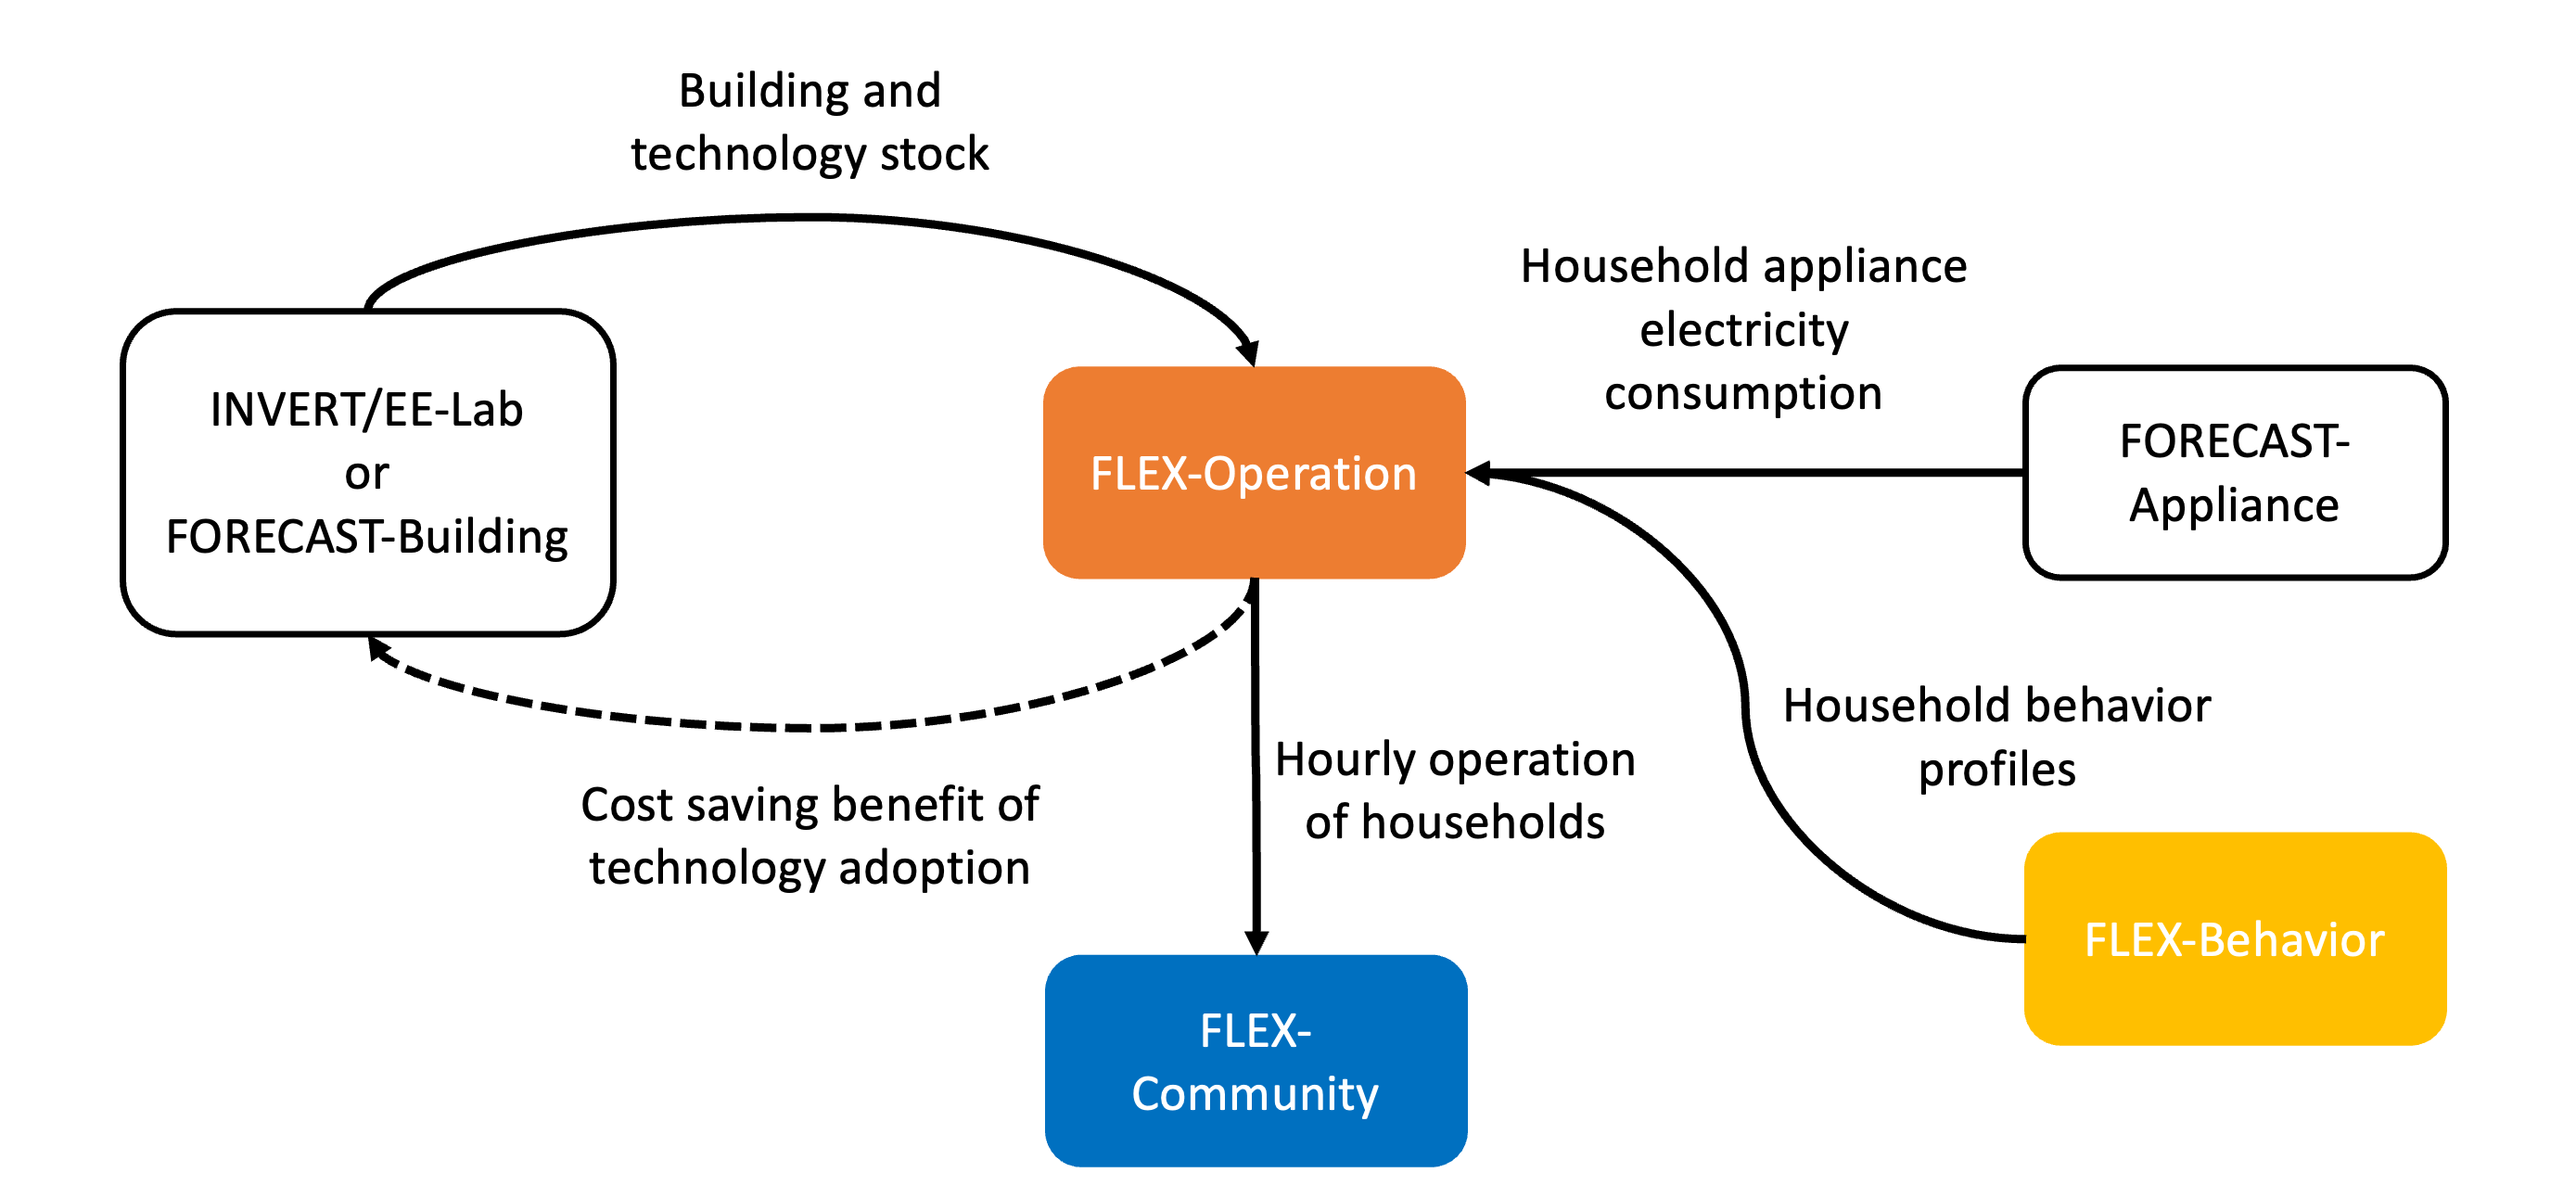
\includegraphics[width=\textwidth]{Images/flex.png}
  \caption{FLEX modeling suite}
  \label{fig:flex}
\end{figure}

%Renewable energy (\gls{re}) and energy efficiency (\gls{ee}) are two central strategies pursued by the \gls{eu} and its Member States concerning the energy system. 
%In 2019, 80.9\% of our total energy supply still depended on burning fossil fuels, namely 26.8\% coal, 30.9\% oil and 23.2\% natural gas \cite{iea}. 
%Investments into low-carbon power generation accounted for 15\% recently are expected to rise to more than 30\% by 2030, corresponding to a quadrupling in absolute volumes \cite{shift}. Solar, wind, and the investments for enabling the integration of these technologies to the grid dominate the investments into low-carbon power generation \cite{shift}. 
%Electrification is playing a major role in the energy transition process. 
%Meanwhile, different electrification strategies rely heavily on energy efficiency \cite{electrification}.
%Measures to increase energy efficiency, including investments in energy savings and the consolidation of consultancy and information services, are promoted by The National Action Plan on Energy Efficiency (\gls{nape}) \cite{bafa}.  

%Transitioning towards a sustainable energy system necessitates significant effort on both the demand and supply sides. 
%However, previous research has shown that in many areas energy efficiency gains were counteracted by societal trends that increased corresponding activities, leading to much smaller decreases (or even increases) of energy demand than technologically feasible \cite{2050}. 
%The aim of newTRENDs is to increase the qualitative and quantitative understanding of impacts of new societal trends on energy consumption and to improve the modelling of energy demand, energy efficiency and policy instruments \cite{fraunhofer}. 


\subsection{The FLEX-Operation model}

The FLEX-Operation model \cite{newtrends} enables the detailed simulation of energy system operation for individual households at an hourly resolution. 
This model provides a comprehensive assessment of the energy consumption of a representative building, incorporating technology operation (such as battery, \gls{pv}, and \gls{hp} systems) and load profiles at an hourly resolution. 
In addition to its capability of modeling energy system operation, FLEX-Operation can also aid in investment decision-making by evaluating the energy-saving benefits associated with technology adoption.

As shown in Figure \ref{fig:flex-operation}, FLEX-Operation considers following services:

%\begin{enumerate}
%  \item electric appliances, e.g., television, refrigerator, lighting, etc.;
%  \item space heating;
%  \item domestic hot water;
%  \item space cooling;
%  \item vehicle. 
%\end{enumerate}

\begin{figure}[h]
  \centering
  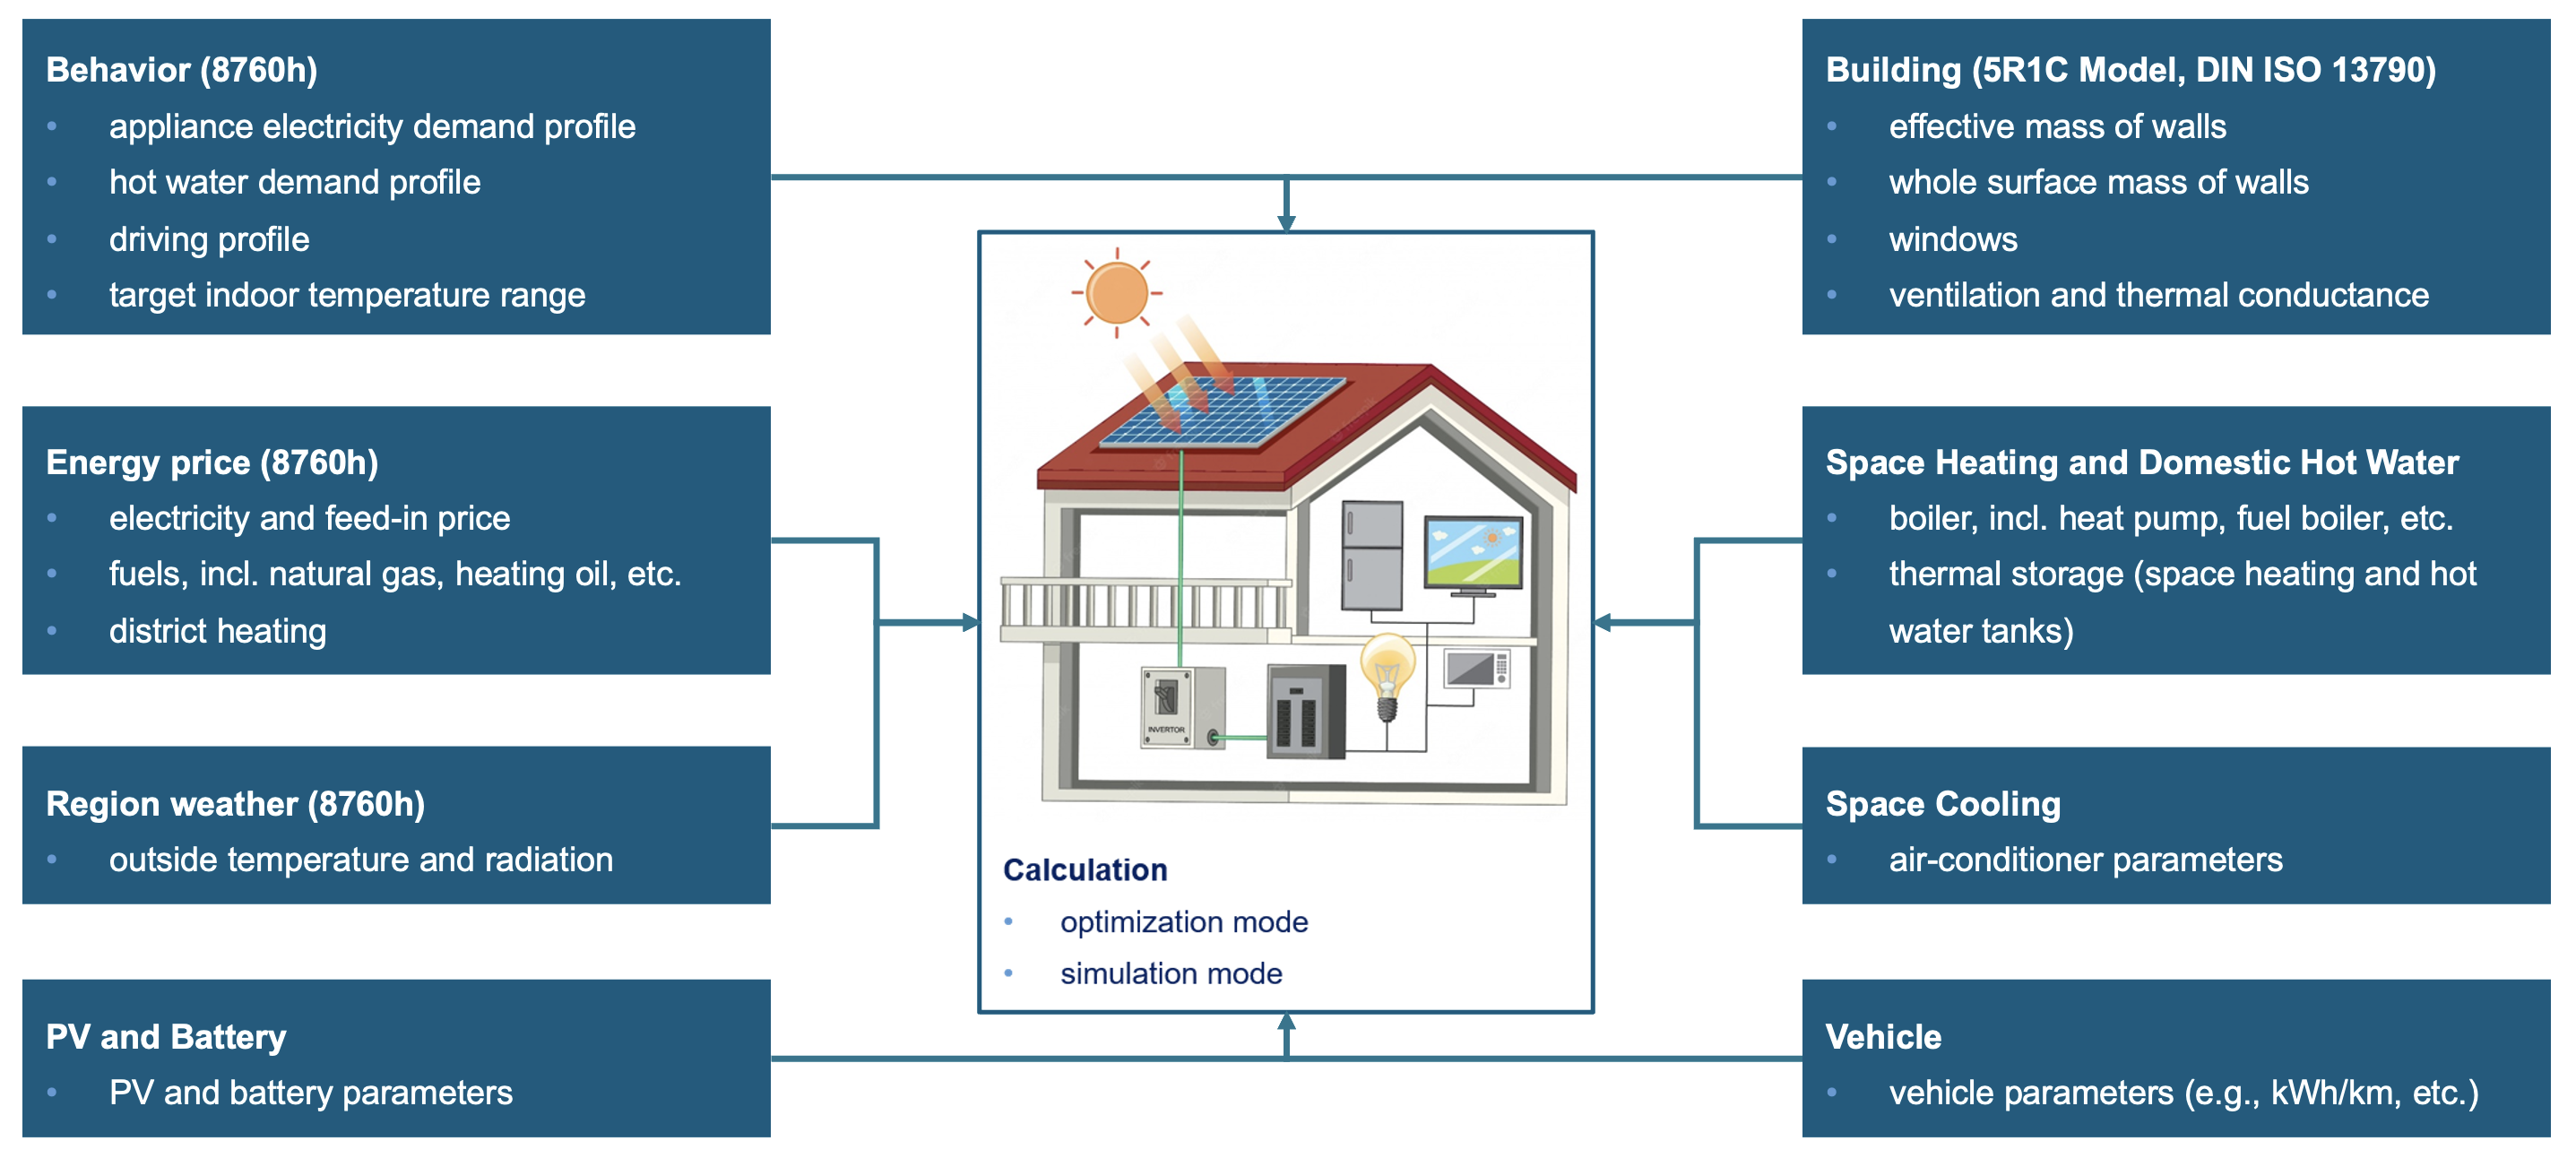
\includegraphics[width=\textwidth]{Images/flex-operation.png}
  \caption{Model structure for individual households}
  \label{fig:flex-operation}
\end{figure}

%Researchers believe new societal trends have the potential to shift energy demands between sectors and might reinforce or diminish one another when they occur at the same time \cite{2050}. 
%Researchers and organisations are paying increasing attention to how new societal trends are affecting energy demand.
%It is therefore important to access current and (foreseeable) future societal trends concerning the impact that they might have on future energy demand \cite{2050}. 

%Four arising societal trend clusters that are likely to shape future energy demand in European countries (and worldwide) were established by Brugger et al. \cite{2050}:  
%\emph{
%  (1) the digitalization of the economy and of private life; 
%  (2) new social and economic models, including the sharing economy and prosumaging (combination of producing, consuming and managing of energy); 
%  (3) industrial transformation, including decarbonization of industrial processes and the circular economy (including a stronger focus on material efficiency); 
%  (4) quality of life, including health effects, urbanization and regionalization. 
%}

%\begin{itemize}
%  \item \textbf{Digitalization of life} %\\ the digitalization of the economy and of private life;
%  \item \textbf{New social and economic models} %\\ including the sharing economy and prosumaging (combination of producing, consuming and managing of energy);
%  \item \textbf{Industrial transformation} %\\ including decarbonization of industrial processes and the circular economy (including a stronger focus on material efficiency);
%  \item \textbf{Quality of life} %\\ including health effects, urbanization and regionalization. 
%\end{itemize}

%The newTRENDs project develops the analytical basis for a “2050 Energy Efficiency Vision” by considering new societal trends in energy demand modeling \cite{newtrends}. 
%Considering the impact of these new societal trends on energy demand from a closer sectoral perspective,
%Yu et al. \cite{newtrends} identified four energy sectors: 

%\begin{itemize}
%  \item industry, 
%  \item transport,  
%  \item tertiary, 
%  \item residential.  
%\end{itemize}

%This proposed thesis will focus on the residential sector while taking scenarios of “consumers” becoming “prosumers” (with \gls{pv}) and “prosumagers” (adding energy storage and \gls{sems}) \cite{consumer} into account.  



\subsection{The FLEX-Behaviour model}

The FLEX-Behaviour model \cite{newtrends} facilitates the modeling of household behavior, including activity profiles and corresponding load profiles. 
By generating an hourly activity and energy demand profile for a pre-defined household, this model provides a comprehensive assessment of the energy consumption patterns of an individual household.

The estimates generated by the FLEX-Behaviour model refer to: 
\begin{itemize}
  \item appliance electricity demand,
  \item domestic hot water demand,
  \item driving profile, and
  \item building occupation.
\end{itemize}

%\subsubsection{INVERT/EE-Lab and FORECAST-Appliance}

%INVERT/EE-Lab and FORECAST-Appliance are the two models that can cover the energy consumption of residential buildings. The two models complement each other and cover the total energy consumption of households. 
%However, both INVERT/EE-Lab and FORECAST-Appliance calculate the energy consumption at the annual resolution and cannot model the prosumaging behavior and energy community, which requires an hourly resolution to consider the impact of household behavior, \gls{pv} generation, and energy storage (thermal and battery) on energy consumption. 
%In this regard, the FLEX-Operation and FLEX-Community models were developed to improve the building modeling suite and support relevant policy analysis \cite{newtrends}. 

%\subsubsection{FLEX-Community}

%FLEX-Community models the operation of an energy community, i.e., household interaction, aggregator optimisation. 
%It can be applied to support the aggregators designing and evaluating business models, as well as making investment decisions, for example, the self-owned battery, \gls{pv} panels, etc. \cite{newtrends}.

\chapter{Design} 

In order to bridge the information gap regarding home energy systems, this study aims to provide households with knowledge of available technologies in the market. 
To address the potential issue of information overload, the study proposes a home energy system recommender to present households with a tailored selection of technologies that better fit their unique home situations, 
such as by learning the location of the house, in order to estimate the amount of sunlight it is likely to receive over the course of a year, to evaluate whether installing a \gls{pv} system would be a viable and effective way for the household.
The learning theory suggests that individuals learn new knowledge by connecting it with existing knowledge and experiences, as this helps to create a framework for understanding and retention of the new information.
Therefore, by focusing on personalised recommendations, the study hypothesises that households may be more receptive to learning about home energy technologies. 
Additionally, with the intention of nudging house owners towards making informed decisions. 

\section{Design concept}
The design concept of the home energy system recommender involves the utilisation of personalised recommendations based on the unique situations of households. 
By gaining a deep understanding of the household's energy demands and supply dynamics, the recommender can offer tailored recommendations to optimise energy efficiency and costs. 
Through this approach, the recommender not only provides guidance on these technologies but also educates the house owners on the potential benefits of transitioning to more sustainable energy sources. 
To ensure the effectiveness of the recommendations, clear and concise explanations are provided to enable users to make informed decisions.


\section{Input to the system}


\subsection{Household profiles}

The concept of household profile has been developed to gain insights into the energy demand and supply dynamics of households. 
To ensure the accuracy of this profile, various factors that may impact the household's energy consumption must be taken into consideration, as shown in Figure \ref{fig:profile}, including 
\emph{
    the external environment, 
    building materials, 
    energy consumption behaviors, 
    and the current home energy system. 
}
By creating such a profile, a comprehensive understanding of the household's situation can be attained, enabling the offering of more tailored and effective recommendations.
\begin{figure}[h]
    \centering
    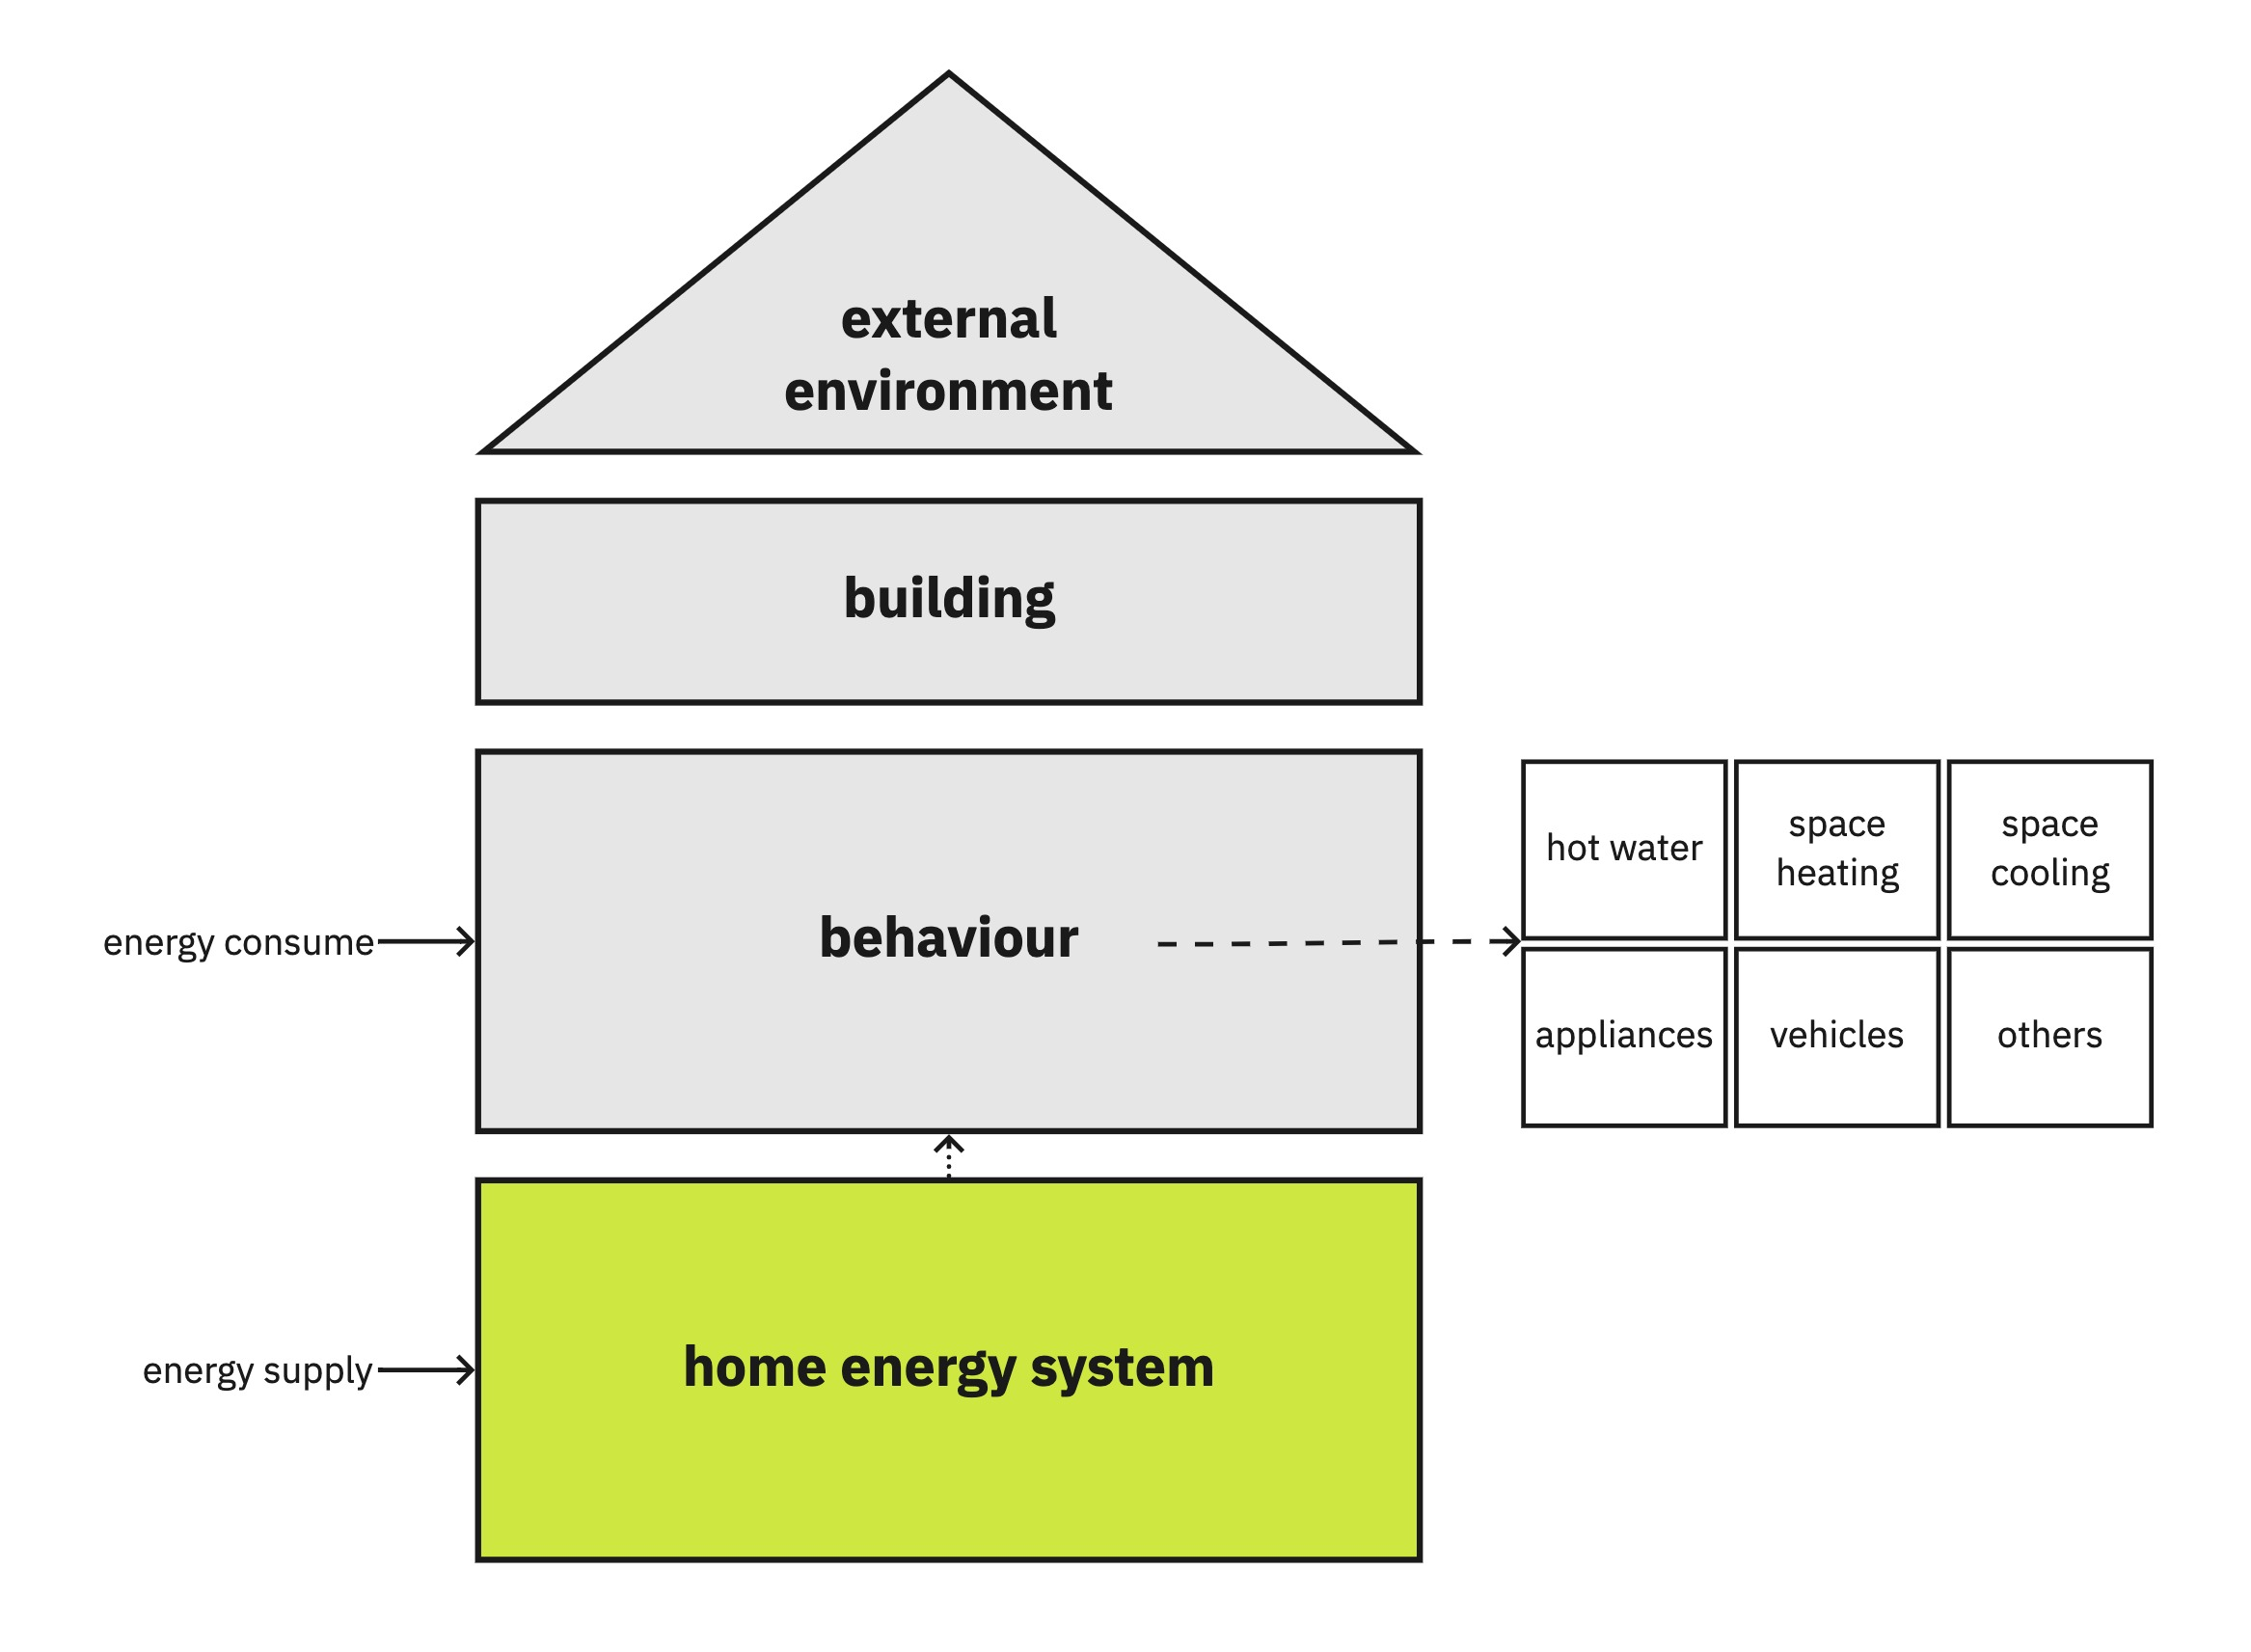
\includegraphics[width=\textwidth]{Images/household_profile.jpg}
    \caption{Household profile}
    \label{fig:profile}
  \end{figure}

\subsubsection{Input data by FLEX models}

In order to accurately anticipate household's energy costs,
the FLEX-Operation model takes a set of variables into account,
and they can be divided into following 15 categories: 
\emph{
    behaviour profile,
    battery,
    behaviour, 
    boiler,
    building,
    energy price,
    heating element, 
    hot water tank,
    \gls{pv},
    region,
    space cooling technology,
    space heating tank,
    vehicle,
    energy price,
    region weather. 
}
Furthermore, the specific data required by the FLEX-Operation model within each category can be found in Appendix \ref{appendix:inputdata}. 


\subsection{Decision trees for asking questions}

A total of 14 questions, see Table \ref{tab:questions}, were raised to collect all the relevant information necessary for the household profile analysis. 
In order to optimise the user experience, a decision tree approach was employed, allowing users to navigate through the questionnaire without the need to answer all the questions. 

\begin{center}
    \small
    \begin{longtable}{ | p{.15\textwidth} | p{.35\textwidth} | p{.35\textwidth} | }
        \hline
        Category & Question & Note \\
        \hline
        External environment & Where is the house located? & Understanding the location of the house can provide valuable insight into its environmental factors, such as the amount of sunlight it receives. \\
        \hline
        House condition & When was the house built? & Knowing the year a house was built can provide insight into its construction materials, such as the composition of the walls. \\
          & Has the house ever been renovated before? & Renovations can include upgrading insulation, replacing windows with energy-efficient ones, installing high-efficiency HVAC systems, sealing air leaks, etc. \\
          & What have been renovated in the house? &   \\
        \hline
        Energy use & How many people are living in the house? &   \\
          & How often does each adult work from home? &   \\
          & Is there any air conditioner in the house? &   \\
          & What type of heating energy is used in the house? &   \\
        \hline
        Home energy system  & Is there a photovoltaic (PV) system in the House? & A PV system is a system that uses solar panels to convert sunlight into electricity for use in a building. \\    
          & What is the size of the \gls{pv} system? &  The average size of a \gls{pv} system is 5 kilowatt-peak. \\
          & Is there a battery system in the house? & A home battery system is a device that stores energy produced by solar panels or other sources to be used later when needed. \\
          & What is the capacity of the battery? & The average capacity of a home battery system is around 7 kilowatt-hours. \\
          & Is there a smart energy management system in the house? &   \\
        \hline
    \caption{Survey questions}
    \label{tab:questions}
    \end{longtable}
\end{center}



\section{Output to the system}

\subsection{Recommendations}

An effective home energy system should prioritize minimizing energy waste, reducing dependence on non-renewable fossil fuels, and lowering overall energy costs. Our recommendations are aligned with these fundamental principles and aim to promote sustainable energy practices while also reducing household energy expenditures. 

The objectives of the recommendation system are multi-fold. 
Firstly, the system aims to support homeowners in making informed decisions regarding investments in home energy systems. 
Additionally, the system intends to encourage behavior change among homeowners by promoting the utilization of renewable energy sources. 
Finally, the recommendation system seeks to continuously refine and improve the accuracy of its predictive model, ensuring that the recommendations provided are up-to-date and effective. 
By providing users with tailored recommendations, the system aims to facilitate the adoption of energy technologies, ultimately leading to reduced energy demand and associated costs. 

As noted by Karen Palmer et al. \cite{informationgap}, financial considerations are of primary importance to homeowners when making decisions about energy investments. 
In line with this understanding, the recommendation system places a strong emphasis on providing transparent cost estimates for energy bills as well as recommended home energy system configurations. 
Additionally, the system seeks to encourage behavior change by providing information and education on climate change and renewable energy sources, aimed at increasing user awareness and understanding of the benefits of sustainable energy practices. 
To facilitate ongoing improvement and refinement of the recommendation system, a feedback survey button will be incorporated, allowing users to provide both short-term and long-term feedback on the system's performance and recommendations. 

\subsection{Explainability}

In order to provide more comprehensive and understandable recommendations, we have chosen to explain our recommendations from multiple perspectives beyond just cost estimates. 
Specifically, we have identified 4 key objectives, including \emph{trust, effectiveness, education, and debugging}, as key aspects to incorporate into our explanations. 
\emph{Trust}, we build trust with our users by using reliable data sources and providing transparent services. 
\emph{Effectiveness}, we strive to enhance the effectiveness of our service by offering recommendations that could actually benefit users economically. 
\emph{Education}, we seek to educate our users on the importance of environmental protection by sharing relevant knowledge and insights. 
\emph{De-bugging}, we value user feedback as an important tool for identifying and resolving any issues or bugs in our system, allowing us to continuously improve and refine our service.
The reasons for offering such explanations are to familiarise users with these technologies, establish accountability in the decision-making process, and encourage a shift towards environmentally conscious behaviour.
By incorporating these concepts into our explanations, we aim to provide recommendations that are transparent, trustworthy, understandable, and user-centred. 

Our recommendation system employs a three-level explainability framework to enhance user understanding of the recommended home energy system configurations. 
At the first level, the system provides an explanation in terms of the expected energy bill for the household. 
At the second level, the system offers a behavioural explanation of energy consumption patterns and the factors driving them. 
Finally, at the third level, the system aims to increase users' awareness and understanding of renewable energy and environmental protection.

Furthermore, the explanation is divided into three layers. 
At the first layer, users are provided with a comprehensive summary of their current energy consumption patterns. 
At the second layer, users are introduced to the various functionalities and benefits of the recommended energy technologies, including cost-saving potential and environmental impact. 
Finally, at the last layer, users are presented with simulated energy demand and supply data, allowing them to see the potential energy savings that could result from adopting the recommended configurations. 

Through the implementation of a comprehensive approach to explainability, our objective is to offer users an overview of energy technologies, enabling them to gain insight into their energy consumption patterns and to recognize the advantages of shifting towards more sustainable energy systems.


\subsection{Investments}

\begin{center}
    \begin{table}[h]
    \small
        \begin{tabular}{ | p{.30\textwidth} | p{.15\textwidth}  p{.15\textwidth}  p{.15\textwidth}  p{.15\textwidth} | }
            \hline
            Technology & \multicolumn{4}{ c | }{Cost (\euro{})} \\
             & Lowest & Highest & Installation & Maintenance \\
            \hline
            \gls{pv} system & \SI[per-mode=symbol,bracket-unit-denominator = false]{1957,68}{\per\kW}p & \SI[per-mode=symbol,bracket-unit-denominator = false]{2231,76}{\per\kW}p & included & 0 \\
            Battery system & \SI[per-mode=symbol,sticky-per,bracket-unit-denominator = false]{790,80}{\per\kWh}  & \SI[per-mode=symbol,sticky-per,bracket-unit-denominator = false]{2520,00}{\per\kWh} & included & 0 \\
            \gls{sems} & / & 1516,11 & 379,03 & 0 \\
            \gls{hp}& \SI[per-mode=symbol,bracket-unit-denominator = false]{432,15}{\per\kW} & \SI[per-mode=symbol,bracket-unit-denominator = false]{2370,31}{\per\kW} & included & 0 \\
            Hot water tank & 1 & 1 & 1 & 0 \\
            Space heating tank & 1 & 1 & 1 & 0 \\
            Air conditioner & 1 & 1 & 1 & 0 \\
            Basement renovation & \SI[per-mode=symbol]{132,12}{\per\metre\squared} & \SI[per-mode=symbol]{157,64}{\per\metre\squared} & included & 0 \\
            Roof renovation & \SI[per-mode=symbol]{40,95}{\per\metre\squared} & \SI[per-mode=symbol]{409,38}{\per\metre\squared} & included & 0 \\
            Wall renovation & \SI[per-mode=symbol]{67,57}{\per\metre\squared} & \SI[per-mode=symbol]{408,93}{\per\metre\squared} & included & 0 \\
            Window renovation & \SI[per-mode=symbol]{364,63}{\per\metre\squared} & \SI[per-mode=symbol]{958,92}{\per\metre\squared} & included & 0 \\
            \hline
        \end{tabular}
    \caption{Investment costs of different technologies}
    \label{tab:investments}
    \end{table}
\end{center}


\section{Interactions}

\subsection{Interfaces}

To facilitate user understanding of the recommended home energy system configurations and associated costs, our recommendation system will employ a visual and natural language explanation interface. 
Specifically, an interactive visualization tool will be implemented to enable users to explore and compare different energy system configurations in terms of energy consumption patterns and costs. 
Additionally, natural language explanations will be provided to further enhance user understanding and engagement with the recommended configurations. 


\subsection{Data visualisation}



\chapter{Development} 

The web application is designed, 
with the frontend responsible for collecting user data and presenting recommendations and explanations, 
while the backend handles the database generated by the FLEX models. 


\section{Frontend}

The frontend of the web application is responsible for creating an engaging and user-friendly interface using HTML, CSS, and JavaScript. 
They were used to structure the content, define the visual styles, and add interactivity to the application.
HTML is used to create the structure of the webpages, CSS is employed to style the visual appearance of the application. 
JavaScript plays a crucial role in adding interactivity and dynamic functionality to the web application. 
Additionally, JavaScript is responsible for making asynchronous requests to the server, facilitating communication with the backend.
To ensure a responsive design, the web application utilises the Bootstrap framework. 
Although the service is not intended for mobile screens, a responsive user interface that adapts to various devices and screen sizes has been taken into account. 


\subsection{Questionnaire}

To incorporate questionnaires into the web application, we integrated SurveyJS, an open-source JavaScript form builder library \cite{surveyjs}. 
SurveyJS simplifies the process of creating and embedding surveys.
It supports logic and branching, allowing for dynamic survey behaviour based on user responses, 
that fulfils our need of presenting corresponding questions according to the answers, as decribed in the design section. 


\subsection{Charts}

For chart building, we initially opted for Google Charts, a charting library provided by Google \cite{googlecharts}. 
However, we encountered difficulties in building multiple columns using Google Charts. 
As a result, we switched to Highcharts \cite{highcharts}, another powerful charting library written in JavaScript. 


\section{Backend}

The backend of the web application utilises Flask, a Python-based web framework \cite{flask}, to serve as the intermediary between the frontend and the FLEX models. 
This choice was made based on the fact that the FLEX models are implemented in Python. 
Originally, our intention was to enable direct communication between the backend and the models using Python. 
However, during the development process, we realised that the models' calculations, especially when finding recommended configurations, could be time-consuming. 
Each scenario takes approximately seven seconds to calculate, and considering the need to identify multiple scenarios that could save energy costs for the household, 
it would be impractical to make the user wait for the results. 
To address this issue, we decided to pre-process the data in the FLEX models and store it in a database. 
This approach significantly reduced the time required to identify energy-saving scenarios, allowing for a more efficient user experience.


\subsection{JSON Schema Documentation}

The API design for the service follows a RESTful architecture and adheres to the JSON schema presented in this section. 
This JSON schema defines the structure and properties of a household's energy system and recommendation.


\subsubsection{Household's energy system and recommendation}


\subsubsection{Properties}

The documentation consists of three main components: profile, current, and recommendation as displayed in table \ref{tab:properties}. 

\begin{table}[h!]
    \centering
    \small
    \begin{tabular}{ | p{.10\textwidth} | p{.10\textwidth} | p{.35\textwidth} | p{.10\textwidth} | p{.10\textwidth} | } 
      \hline
      Name & Type & Description & Required & Default value \\
      \hline
      profile & object & An object describing the house's location and number of people. & Yes & - \\
      \hline
      current & object & An object describing the house's current energy system configurations, energy data, and costs. & Yes & - \\
      \hline
      recom-men-dation & array & A list of recommended configurations that improve the house's energy efficiency. & Yes & - \\
      \hline
    \end{tabular}
    \caption{Properties}
    \label{tab:properties}
\end{table}


\subsubsection{Properties of profile}

As table \ref{tab:properties_profile} shows, the profile component provides information about the house's location and the number of people residing in it. 
It includes properties such as location and person.

\begin{table}[h!]
    \centering
    \small
    \begin{tabular}{ | p{.10\textwidth} | p{.10\textwidth} | p{.35\textwidth} | p{.10\textwidth} | p{.10\textwidth} | } 
    \hline
    Name & Type & Description & Required & Default value \\
    \hline
    location & string & The location of the house. & Yes & - \\
    \hline
    person & integer & The total number of people residing in the house. & Yes & - \\
    \hline
    \end{tabular}
    \caption{Properties of profile}
    \label{tab:properties_profile}
\end{table}


\subsubsection{Properties of current}

The current component describes the house's current energy system configurations, energy data, and costs. 
It consists of two properties: config and energy\_data. 
See table \ref{tab:properties_current}.

\begin{table}[h!]
    \centering
    \small
    \begin{tabular}{ | p{.10\textwidth} | p{.10\textwidth} | p{.35\textwidth} | p{.10\textwidth} | p{.10\textwidth} | } 
    \hline
    Name & Type & Description & Required & Default value \\
    \hline
    config & object & An object describing the house's current energy system configurations. & Yes & - \\
    \hline
    \makecell{energy\_\\data} & object & An object describing the energy demand, PV generation, and energy cost. & Yes & - \\
    \hline
    \end{tabular}
    \caption{Properties of current}
    \label{tab:properties_current}
\end{table}


\subsubsection{Properties of config}

The config property, as shown in table \ref{tab:properties_config}, captures the current energy system configurations, including parameters such as pv\_size, battery\_capacity, sems, heating\_system, heating\_system\_type, and building\_renovation.

\begin{table}[h!]
    \centering
    \small
    \begin{tabular}{ | p{.10\textwidth} | p{.10\textwidth} | p{.35\textwidth} | p{.10\textwidth} | p{.10\textwidth} | } 
    \hline
    Name & Type & Description & Required & Default value \\
    \hline
    pv\_size & integer & Determine the size of the PV system. & Yes & - \\
    \hline
    \makecell{battery\_\\capacity} & integer & Determine the capacity of the battery system. & Yes & - \\
    \hline
    sems & boolean & Determine the state of a SEMS system. & Yes & - \\
    \hline
    \makecell{heating\_\\system} & boolean & Determine the state of the heating system used.	 & Yes & - \\
    \hline
    \makecell{boiler\_\\type} & string & Determine the type of heating system used. & Yes & - \\
    \hline
    \makecell{building\_\\renovation} & boolean & Determine the state of the renovation. & Yes & - \\
    \hline
    \end{tabular}
    \caption{Properties of config}
    \label{tab:properties_config}
\end{table}


\subsubsection{Properties of energy\_data}

The energy\_data property contains data related to energy demand, PV generation, and energy cost. 
It includes properties like energy\_demand, energy\_generate, heating, cooling, appliance, hotwater, pv, and energy\_bill\_year.
See table \ref{tab:properties_energydata}. 

\begin{table}[h!]
    \centering
    \small
    \begin{tabular}{ | p{.10\textwidth} | p{.10\textwidth} | p{.35\textwidth} | p{.10\textwidth} | p{.10\textwidth} | } 
    \hline
    Name & Type & Description & Required & Properties in Database \\
    \hline
    \makecell{energy\_\\demand} & integer & The total energy demand in a year. & Yes & - \\
    \hline
    \makecell{energy\_\\generate} & integer & The total energy generated by PV in a year. & Yes & - \\
    \hline
    heating & array & The energy demanded for heating in the house for each month. & Yes & \makecell{E\_\\Heating\_\\HP\_out \\+ Q\_\\Heating\\Element} \\
    \hline
    cooling & array & The energy demanded for cooling in the house for each month. & Yes & \makecell{E\_\\Room\\Cooling} \\
    \hline
    appliance & array & The energy demanded by all appliances in the house for each month. & Yes & \makecell{BaseLoad\\Profile} \\
    \hline
    hotwater & array & The energy demanded for hot water in the house for each month. & Yes & \makecell{E\_DHW\_\\HP\_out} \\
    \hline
    pv & string & The energy generated from PV in the house for each month. & Yes & \makecell{Photo\\voltaic\\Profile} \\
    \hline
    \makecell{energy\_\\bill\_\\year} & integer & The total yearly energy cost. & Yes & - \\
    \hline
    \end{tabular}
    \caption{Properties of energy\_data}
    \label{tab:properties_energydata}
\end{table}


\subsubsection{Properties of recommendation}

The recommendation component represents a list of recommended configurations that can improve the house's energy efficiency. 
As listed in table \ref{tab:properties_recommendation}, each recommendation includes properties similar to the config and energy\_data properties in the current component. 
Additionally, it includes an investment\_cost property indicating the annualised investment cost for the recommended configuration. 

\begin{table}[h!]
    \centering
    \small
    \begin{tabular}{ | p{.10\textwidth} | p{.10\textwidth} | p{.35\textwidth} | p{.10\textwidth} | p{.10\textwidth} | } 
    \hline
    Name & Type & Description & Required & Default value \\
    \hline
    config & object & An object describing the recommended energy system configurations. & Yes & - \\
    \hline
    \makecell{energy\_\\data} & object & An object describing the energy demand, PV generation, and energy cost. & Yes & - \\
    \hline
    \makecell{investm\\ent\_cost} & integer & The annualised investment cost for the recommended configuration. & Yes & - \\
    \hline
    \end{tabular}
    \caption{Properties of recommendation}
    \label{tab:properties_recommendation}
\end{table}


\subsubsection{Example JSON data}

\begin{verbatim}
"energy_data": {
    "total_generate": <int>,
    "total_demand": <int>,
    "boiler": <int[12]>,
    "cooling": <int[12]>,
    "appliance": <int[12]>,
    "hotwater": <int[12]>,
    "pv": <int[12]>
},
\end{verbatim}

The JSON data example can be found in the appedix \ref{appendix:example_JSON}. 

\subsection{Endpoints}

The API exposes five endpoints to retrieve data,
they are survey\_scenario, scenario, recommendation, energy\_data, and eenergy\_cost.
The endpoints accept HTTP GET requests and returns JSON responses. 

\appendix

\appendixpage
\addappheadtotoc
\chapter{Input of the FLEX models}
\label{appendix:inputdata}

\begin{center}
    \small
    \begin{longtable}{ | p{.10\textwidth} | p{.80\textwidth} | }
        \hline 
        \multicolumn{1}{|c|}{\textbf{Category}} & \multicolumn{1}{c|}{\textbf{Data}} \\ 
        \hline 
        \endfirsthead

        \multicolumn{2}{l}
        {{\bfseries \tablename\ \thetable{} -- continued from previous page}} \\
        \hline \multicolumn{1}{|c|}{\textbf{Category}} &
        \multicolumn{1}{c|}{\textbf{Data}} \\  
        \endhead

        \multicolumn{2}{|r|}{{Continued on next page}} \\ 
        \hline
        \endfoot

        \endlastfoot
            Behaviour profile & id\_hour, people\_at\_home\_profile\_1, hot\_water\_demand\_profile\_1, appliance\_electricity\_demand\_profile\_1, vehicle\_at\_home\_profile\_1, vehicle\_distance\_profile\_1. \\
            \hline 
            Battery & ID\_Battery, capacity, capacity\_unit, charge\_efficiency, charge\_power\_max, charge\_power\_max\_unit, discharge\_efficiency, discharge\_power\_max, discharge\_power\_max\_unit. \\
            \hline 
            Behaviour & ID\_Behavior, id\_people\_at\_home\_profile, target\_temperature\_at\_home\_max, target\_temperature\_at\_home\_min, target\_temperature\_not\_at\_home\_max, target\_temperature\_not\_at\_home\_min, shading\_solar\_reduction\_rate, shading\_threshold\_temperature, temperature\_unit, id\_hot\_water\_demand\_profile, hot\_water\_demand\_annual, hot\_water\_demand\_unit, id\_appliance\_electricity\_demand\_profile, appliance\_electricity\_demand\_annual, appliance\_electricity\_demand\_unit, id\_vehicle\_at\_home\_profile, id\_vehicle\_distance\_profile. \\
            \hline 
            Boiler & ID\_Boiler, type, power\_max, power\_max\_unit, carnot\_efficiency\_factor. \\
            \hline 
            Building & ID\_Building, type, construction\_period\_start, construction\_period\_end, person\_num, Af, Hop, Htr\_w, Hve, CM\_factor, Am\_factor, internal\_gains, effective\_window\_area\_west\_east, effective\_window\_area\_south, effective\_window\_area\_north, grid\_power\_max, supply\_temperature. \\
            \hline
            Energy price & ID\_EnergyPrice, id\_electricity, id\_electricity\_feed\_in, id\_gases, price\_unit. \\
            \hline
            Heating element & ID\_HeatingElement, power, power\_unit, efficiency. \\
            \hline 
            Hot water tank & ID\_HotWaterTank, size, size\_unit, surface\_area, surface\_area\_unit, loss, loss\_unit, temperature\_start, temperature\_max, temperature\_min, temperature\_surrounding, temperature\_unit. \\
            \hline 
            \gls{pv} & ID\_PV, size, size\_unit. \\
            \hline
            Region & ID\_Region, code, year, norm\_outside\_temperature. \\
            \hline 
            Space cooling technology & ID\_SpaceCoolingTechnology, efficiency, power, power\_unit. \\
            \hline 
            Space heating tank & ID\_SpaceHeatingTank, size, size\_unit, surface\_area, surface\_area\_unit, loss, loss\_unit, temperature\_start, temperature\_max, temperature\_min, temperature\_surrounding, temperature\_unit. \\
            \hline 
            Vehicle & ID\_Vehicle, type, capacity, capacity\_unit, consumption\_rate, consumption\_rate\_unit, charge\_efficiency, charge\_power\_max, charge\_power\_max\_unit, discharge\_efficiency, discharge\_power\_max, discharge\_power\_max\_unit, charge\_bidirectional. \\
            \hline 
            Energy price & Region, year, id\_hour, electricity\_1, electricity\_2, electricity\_feed\_in\_1, gases\_1. \\
            \hline 
            Region weather & region, year, id\_hour, pv\_generation, pv\_generation\_unit, temperature, temperature\_unit, radiation\_south, radiation\_east, radiation\_west, radiation\_north, radiation\_unit. \\
            \hline 
        \caption{Input data of the FLEX-Operation model}
        \label{tab:inputdata}
    \end{longtable}
\end{center}

\nocite{*} % Without this, only cited materials are displayed in the bibliography.

\bibliographystyle{thesnumb}
\bibliography{ref}

%Written insurance
\clearpage % Start a new page

\noindent

I certify that I have prepared the written elaboration independently and have not used any other aids than those specified. All passages that are taken from other works in terms of wording or meaning (including translations) have been clearly identified as borrowing in each individual case, giving precise details of the source (including the World Wide Web and other electronic data collections). This also applies to attached drawings, pictorial representations, sketches and the like. I acknowledge that the proven omission of the indication of origin will be assessed as an attempted deception.

\end{document}
